\documentclass[10pt]{beamer}

% --- Theme & Colors ---
\usetheme{Madrid}
\usecolortheme{default}
\setbeamertemplate{navigation symbols}{}
\setbeamertemplate{footline}{\hfill\insertframenumber/\inserttotalframenumber\hspace*{5pt}\vspace{2pt}}

% --- Packages ---
\usepackage{amsmath,amssymb}
\usepackage{graphicx}
\usepackage{booktabs}
\usepackage[table]{xcolor}
\usepackage{tikz}
\usetikzlibrary{shapes,arrows.meta,positioning,fit,calc}

% --- Custom Colors ---
\definecolor{neuralblue}{RGB}{30,90,160}
\definecolor{spikegreen}{RGB}{34,139,34}
\definecolor{contriborange}{RGB}{210,105,30}

\setbeamercolor{structure}{fg=neuralblue}
\setbeamercolor{block title}{bg=neuralblue,fg=white}
\setbeamercolor{block body}{bg=blue!5}
\setbeamercolor{block title alerted}{bg=red!70!black,fg=white}
\setbeamercolor{block title example}{bg=spikegreen,fg=white}

% --- Math operators ---
\DeclareMathOperator*{\argmin}{arg\,min}
\DeclareMathOperator*{\argmax}{arg\,min}

% ============================================================
\title{Adaptive EEG-to-Spike Framework}
\subtitle{Energy-Efficient Motor Imagery Decoding on Spiking Neural Networks}
\author{
  Bala Mosay J \quad (2023BTIA029) \\[2pt]
  \textit{Team Member:} Allwyn Jeffo Raj A \quad (2023BTIA002)
}
\institute{Under the guidance of Dr.\ Vaibhav Meshram}
\date{3rd Review --- September 2, 2026}

\begin{document}

% ============================================================
\begin{frame}
\titlepage
\end{frame}

% ============================================================
\begin{frame}{Motivation \& Pipeline Overview}

\begin{columns}[T]
\begin{column}{0.45\textwidth}
\footnotesize
\textbf{Problem:} EEG decoders (CNN/RNN) are too slow for edge devices.

\vspace{2pt}
\textbf{Solution:} Spiking Neural Networks---event-driven, ultra-low power.

\vspace{2pt}
\textbf{Three Gaps:}
\begin{enumerate}
  \item Fixed bands ignore subject-specific rhythms
  \item Fixed thresholds waste energy
  \item Single-timescale neurons miss multi-scale dynamics
\end{enumerate}
\end{column}
\begin{column}{0.52\textwidth}
\textbf{\small 6-Stage Pipeline:}
\vspace{2pt}
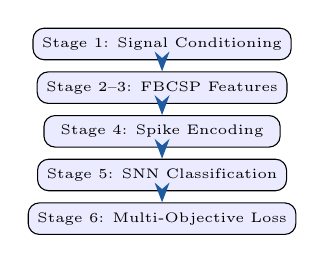
\begin{tikzpicture}[
  node distance=4pt and 0pt,
  box/.style={draw, rounded corners, fill=blue!8, minimum width=3.0cm,
               minimum height=0.4cm, align=center, font=\tiny},
  arrow/.style={-{Stealth[length=2.5mm]}, thick, neuralblue},
]
\node[box] (s1) {Stage 1: Signal Conditioning};
\node[box, below=of s1] (s23) {Stage 2--3: FBCSP Features};
\node[box, below=of s23] (s4) {Stage 4: Spike Encoding};
\node[box, below=of s4] (s5) {Stage 5: SNN Classification};
\node[box, below=of s5] (s6) {Stage 6: Multi-Objective Loss};
\draw[arrow] (s1.south) -- (s23.north);
\draw[arrow] (s23.south) -- (s4.north);
\draw[arrow] (s4.south) -- (s5.north);
\draw[arrow] (s5.south) -- (s6.north);
\end{tikzpicture}
\vspace{2pt}
{\tiny\textcolor{contriborange}{\textbf{C1}} = Adaptive Bands\quad
 \textcolor{contriborange}{\textbf{C2}} = Learnable $\theta$\quad
 \textcolor{contriborange}{\textbf{C3}} = PLIF Network}
\end{column}
\end{columns}

\end{frame}

% ============================================================
\begin{frame}{Stages 1--3: Signal Conditioning \& FBCSP Features}

\footnotesize
\textbf{Stage 1 --- Signal Conditioning:}\\
Bandpass 0.5--40\,Hz $\to$ ICA $\to$ 4\,s epoching $\to$ baseline correction $\to$ per-subject z-score.

\vspace{2pt}
\textbf{Stage 2--3 --- Filter-Bank CSP:}\\
For each band $b$, apply One-vs-Rest CSP, then compute log-variance features:

\vspace{-2pt}
\begin{equation}
\boxed{f_b = \log\!\left(\mathrm{Var}(\hat{x}_b) + \epsilon\right)}
\tag{Eq.~7}
\end{equation}

\vspace{-4pt}
where $\hat{x}_b$ is the CSP-projected signal in band $b$.

\vspace{2pt}
\textbf{Baseline:} $\mu$ (8--12\,Hz), $\beta$ (13--30\,Hz) $\to$ 32 features (2 bands $\times$ 4 classes $\times$ 4 components).

\end{frame}

% ============================================================
\begin{frame}{Contribution 1: Adaptive Band Selection via KNN-MI}

\footnotesize
\textbf{Idea:} Rank frequency bands per-subject using Mutual Information.

\vspace{2pt}
\textbf{Kraskov KNN-MI Estimator:}
\vspace{-2pt}
\begin{equation}
\hat{I}(X; Y) = \psi(k) - \langle \psi(n_x^{(k)} + 1) \rangle + \psi(N) - \psi(K)
\tag{Eq.~8}
\end{equation}

\vspace{-4pt}
where $\psi$ = digamma function, $k$ = KNN parameter, $n_x^{(k)}$ = neighbors sharing class label.

\vspace{2pt}
\textbf{Band Selection:}
\vspace{-2pt}
\begin{equation}
J(B_i) = \hat{I}(B_i;\, Y) \qquad \Longrightarrow \qquad \text{Select top-3 from 7-band bank (4--32\,Hz)}
\tag{Eq.~11}
\end{equation}

\vspace{-2pt}
7 bands of 4\,Hz width, 2\,Hz step $\to$ per-subject top-3 $\to$ personalized features.

\end{frame}

% ============================================================
\begin{frame}{Stage 4: Spike Encoding \& LIF Dynamics}

\footnotesize
\begin{columns}[T]
\begin{column}{0.48\textwidth}
\textbf{Binary Spike Encoding:}
\vspace{-2pt}
\begin{equation}
S(t) = H(|x| - \theta)
\tag{Eq.~12}
\end{equation}

\vspace{-4pt}
$H$ = Heaviside, $\theta$ = firing threshold.

\vspace{2pt}
\textbf{LIF Membrane Dynamics:}
\vspace{-2pt}
\begin{equation}
V[t] = V[t\!-\!1] \cdot (1 - 1/\tau) + X[t]
\tag{Eq.~14}
\end{equation}

\vspace{-4pt}
Spike when $V[t] \geq V_{th}$, then $V \!\leftarrow\! 0$.
\end{column}
\begin{column}{0.48\textwidth}
\textbf{Surrogate Gradient:}\\
$H$ is non-differentiable. Use arctangent approximation:
\vspace{-2pt}
\begin{equation}
\frac{\partial S}{\partial V} \approx \frac{1}{\pi(1 + (\pi(V - V_{th}))^2)}
\tag{Eq.~13}
\end{equation}

\vspace{2pt}
This enables end-to-end backpropagation through the spiking neurons while preserving gradient flow during training.
\end{column}
\end{columns}

\end{frame}

% ============================================================
\begin{frame}{Contribution 2: Learnable Spike Threshold}

\footnotesize
\textbf{Baseline:} Fixed $\theta$ = 75th percentile of training features $\to$ same for all subjects.

\vspace{2pt}
\textbf{Proposed:} $\theta \in \mathbb{R}^+$ as \textbf{learnable parameter} (nn.Parameter), jointly optimized with network weights.

\vspace{2pt}
\textbf{Sparsity Penalty:}
\vspace{-2pt}
\begin{equation}
L_{\text{sparse}} = \frac{1}{N_{\text{neurons}}} \sum_j \bar{s}_j
\tag{Eq.~15--17}
\end{equation}

\vspace{-4pt}
$\bar{s}_j$ = average firing rate of neuron $j$. Weight $\lambda_e$ controls sparsity--accuracy trade-off:

\vspace{-2pt}
\begin{equation}
\lambda_e(t) = \lambda_{\max} \cdot \frac{t}{T_{\text{warm}}}
\tag{Warm-up}
\end{equation}

\vspace{-4pt}
$\lambda_e$ ramps from 0 to $\lambda_{\max}$ over $T_{\text{warm}}$ epochs---learn first, enforce sparsity later.

\end{frame}

% ============================================================
\begin{frame}{Stage 5: Baseline LIF Network Architecture}

\textbf{\small Architecture (standard single-$\tau$ LIF):}

\vspace{2pt}
\begin{center}
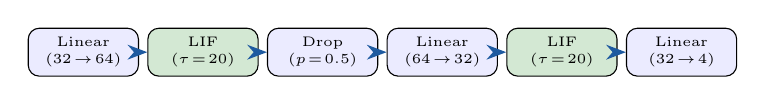
\begin{tikzpicture}[
  node distance=3pt,
  block/.style={draw, rounded corners, fill=blue!8, minimum width=1.4cm,
                 minimum height=0.45cm, align=center, font=\tiny},
  spike/.style={draw, rounded corners, fill=spikegreen!20, minimum width=1.4cm,
                 minimum height=0.45cm, align=center, font=\tiny},
  arrow/.style={-{Stealth[length=2.5mm]}, thick, neuralblue},
]
\node[block] (lin1) {Linear\\$(32\!\to\!64)$};
\node[spike, right=3pt of lin1] (lif1) {LIF\\$(\tau\!=\!20)$};
\node[block, right=3pt of lif1] (drop) {Drop\\$(p\!=\!0.5)$};
\node[block, right=3pt of drop] (lin2) {Linear\\$(64\!\to\!32)$};
\node[spike, right=3pt of lin2] (lif2) {LIF\\$(\tau\!=\!20)$};
\node[block, right=3pt of lif2] (out) {Linear\\$(32\!\to\!4)$};
\draw[arrow] (lin1) -- (lif1);
\draw[arrow] (lif1) -- (drop);
\draw[arrow] (drop) -- (lin2);
\draw[arrow] (lin2) -- (lif2);
\draw[arrow] (lif2) -- (out);
\end{tikzpicture}
\end{center}

\vspace{2pt}
\footnotesize
\textbf{Classification:} Spike-vote---sum output logits over $T\!=\!16$ timesteps, then argmax.

\vspace{-2pt}
\[
\hat{y} = \argmax_{c} \sum_{t=1}^{T} z_c[t]
\]

\end{frame}

% ============================================================
\begin{frame}{Contribution 3: Dual-Branch PLIF with Attention}

\footnotesize
\textbf{Two parallel LIF branches with learnable $\tau$:}

\vspace{2pt}
\begin{center}
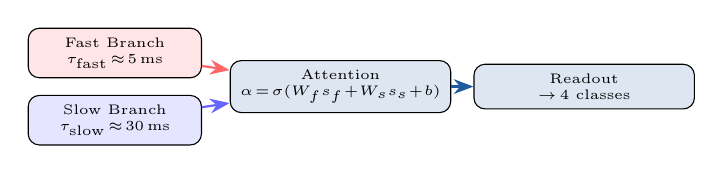
\begin{tikzpicture}[
  node distance=6pt and 10pt,
  branch/.style={draw, rounded corners, minimum width=2.2cm,
                  minimum height=0.4cm, align=center, font=\tiny},
  merge/.style={draw, rounded corners, fill=neuralblue!15, minimum width=2.8cm,
                 minimum height=0.4cm, align=center, font=\tiny},
  arrow/.style={-{Stealth[length=2.5mm]}, thick},
]
\node[branch, fill=red!10] (fast) {Fast Branch\\$\tau_{\text{fast}}\!\approx\!5$\,ms};
\node[branch, fill=blue!10, below=of fast] (slow) {Slow Branch\\$\tau_{\text{slow}}\!\approx\!30$\,ms};
\node[merge, right=10pt of $(fast.east)!0.5!(slow.east)$] (attn) {Attention\\$\alpha\!=\!\sigma(W_f s_f\!+\!W_s s_s\!+\!b)$};
\node[merge, right=8pt of attn] (out) {Readout\\$\to$\,4 classes};
\draw[arrow,red!60] (fast) -- (attn);
\draw[arrow,blue!60] (slow) -- (attn);
\draw[arrow,neuralblue] (attn) -- (out);
\end{tikzpicture}
\end{center}

\vspace{2pt}
\textbf{Membrane dynamics (PLIF):}
\vspace{-2pt}
\begin{equation}
V[t] = V[t\!-\!1] \cdot (1 - 1/\tau) + X[t]
\tag{PLIF}
\end{equation}

\vspace{-4pt}
$\tau$ is \textbf{learnable} per neuron, optimized via surrogate gradients.

\end{frame}

% ============================================================
\begin{frame}{Stage 6: Multi-Objective Loss Function}

\footnotesize
\textbf{Joint loss (Eq.~22--24):}
\vspace{-2pt}
\begin{equation}
\boxed{L = L_{\text{CE}} + \beta \cdot L_{\text{MSE}} + \lambda_e \cdot L_{\text{sparse}} + \gamma \cdot L_{\text{entropy}}}
\tag{Eq.~22}
\end{equation}

\vspace{-2pt}
\begin{tabular}{lll}
\toprule
\textbf{Term} & \textbf{Formula} & \textbf{Purpose} \\
\midrule
$L_{\text{CE}}$ & $-\sum_c y_c \log \hat{y}_c$ & Classification \\
$L_{\text{MSE}}$ & $\frac{1}{C}\sum_c (\hat{y}_c - y_c)^2$ & Soft-label consistency \\
$L_{\text{sparse}}$ & $\frac{1}{N}\sum_j \bar{s}_j$ & Energy efficiency \\
$L_{\text{entropy}}$ & $-\sum_c \hat{y}_c \log \hat{y}_c$ & Class balance \\
\bottomrule
\end{tabular}

\vspace{2pt}
\textbf{Baseline:} Only $L_{\text{CE}}$ ($\lambda_e = 0$). Full model uses all four terms.

\end{frame}

% ============================================================
\begin{frame}{Energy Metric: Synaptic Operations (SynOps)}

\footnotesize
\textbf{Standard energy proxy (Eq.~25):}
\vspace{-2pt}
\begin{equation}
\boxed{\text{SynOps} = \sum_{l=1}^{L} \text{fanout}_l \cdot \bar{s}_l}
\tag{Eq.~25}
\end{equation}

\vspace{-4pt}
\begin{itemize}
  \item $\text{fanout}_l$ = output connections of spiking layer $l$
  \item $\bar{s}_l$ = average spikes per neuron in layer $l$ across $T$ timesteps
\end{itemize}

\vspace{2pt}
\textbf{Interpretation:} Lower SynOps $\Rightarrow$ lower energy on neuromorphic hardware.

\vspace{2pt}
\textbf{Spike density:} $\rho = \frac{1}{L \cdot N \cdot T} \sum_{l,n,t} s_{l,n}[t]$ \quad Target: $\rho \approx 0.10$--$0.20$.

\end{frame}

% ============================================================
\begin{frame}{Evaluation Protocol}

\begin{columns}[T]
\begin{column}{0.48\textwidth}
\footnotesize
\textbf{Dataset:} PhysioNet EEG Motor Movement/Imagery
\begin{itemize}
  \item 109 subjects, 64 channels, 160\,Hz
  \item 4 classes: left hand, right hand, feet, rest
  \item 6 excluded $\to$ \textbf{103 usable subjects}
\end{itemize}

\vspace{2pt}
\textbf{CV Protocol (Sec.~6.2):}
\begin{itemize}
  \item Trial-pooled, subject-mixed 5-fold CV
  \item All parameters fit on train fold only (no leakage)
\end{itemize}
\end{column}
\begin{column}{0.48\textwidth}
\footnotesize
\textbf{Metrics:}
\begin{itemize}
  \item Classification accuracy
  \item Cohen's $\kappa$, Macro F1
  \item SynOps/trial, Spike density
\end{itemize}

\vspace{2pt}
\textbf{Baselines for Comparison:}
\begin{itemize}
  \item SGLNet [8]: Graph CNN + LSTM
  \item Our baseline SNN (fixed bands, fixed $\theta$, single-$\tau$)
\end{itemize}
\end{column}
\end{columns}

\end{frame}

% ============================================================
\begin{frame}{Current Status}

\begin{columns}[T]
\begin{column}{0.48\textwidth}
\footnotesize
\textbf{Phase 1: Signal Conditioning} \checkmark\\
Bandpass, ICA, epoching, AutoReject, z-score. 103 subjects cached.

\vspace{2pt}
\textbf{Phase 2: Baseline SNN} \checkmark\\
\begin{tabular}{lr}
\toprule
\textbf{Classifier} & \textbf{Accuracy} \\
\midrule
SNN (subject-mixed) & 31.8\% $\pm$ 1.1 \\
LogReg (subject-mixed) & 34.6\% $\pm$ 0.8 \\
LogReg (within-subject) & 42.0\% $\pm$ 10.6 \\
\bottomrule
\end{tabular}

\vspace{2pt}
Bottleneck: features (34.6\%), not model. 39/39 tests pass.
\end{column}
\begin{column}{0.48\textwidth}
\footnotesize
\textbf{Key Bugs Fixed:}
\begin{enumerate}
  \item Absolute-value encoding ($|x| > \theta$)
  \item ReLU before LIF removed (standard LIF)
  \item Gradient clipping ($1.0 \to 5.0$)
  \item CSP: \texttt{ledoit\_wolf(X.T)} not \texttt{ledoit\_wolf(cov)}
\end{enumerate}

\vspace{2pt}
\textbf{Bottleneck Analysis:}
\begin{itemize}
  \item Per-subject CSP \textit{are} discriminative (42\%)
  \item Unseen-subject generalization is the challenge (LOSO pending)
  \item Phase 3 contributions address this
\end{itemize}
\end{column}
\end{columns}

\end{frame}

% ============================================================
\begin{frame}{What's Remaining (Phase 3)}

\begin{center}
\footnotesize
\begin{tabular}{cll}
\toprule
\textbf{C\#} & \textbf{Component} & \textbf{Status} \\
\midrule
C1 & Adaptive band selection (KNN-MI) & \textcolor{red}{$\square$~To do} \\
C2 & Learnable spike threshold & \textcolor{red}{$\square$~To do} \\
C3 & Dual-branch PLIF network + attention & \textcolor{red}{$\square$~To do} \\
-- & Joint loss ($L_{CE} + L_{MSE} + L_{sparse} + L_{entropy}$) & \textcolor{red}{$\square$~To do} \\
\midrule
\rowcolor{blue!8}
-- & Signal conditioning (Stage 1) & \textcolor{green!60!black}{$\checkmark$~Done} \\
\rowcolor{blue!8}
-- & FBCSP features (Stage 2--3) & \textcolor{green!60!black}{$\checkmark$~Done} \\
\rowcolor{blue!8}
-- & Baseline SNN evaluation (Stage 4--6) & \textcolor{green!60!black}{$\checkmark$~Done} \\
\bottomrule
\end{tabular}
\end{center}

\vspace{4pt}
\textbf{Target:} Full model accuracy $\geq 55$--$65\%$ with lower SynOps than baseline.

\end{frame}

% ============================================================
\begin{frame}{Thank You}

\begin{center}
\vspace{8pt}
{\Large\textbf{Thank You}}\\[10pt]
{\large Questions \& Discussion}

\vspace{16pt}
\textbf{Team Members:}\\
Bala Mosay J \quad (2023BTIA029)\\
Allwyn Jeffo Raj A \quad (2023BTIA002)

\vspace{8pt}
\textbf{Guide:}\\
Dr.\ Vaibhav Meshram
\end{center}

\end{frame}

\end{document}
